\chapter{Strängars rörelse i vätskor}

%\subsubsection{Strängrörelser inom cellen}
Aktinfilament är polymerer som utgör en viktig byggsten för cellens cytoskelett och transportväg för motorprotein vilka formar och bidrar till cellens utseende, dynamik och stadga. För att kunna ge en mer detaljerad beskrivning av dessa egenskaper är studien av enstaka aktinfilaments dynamik av stort intresse. I detta arbete har olika dynamiska egenskaper för aktinfilament i en miljö utanförcellen studerats, både för filament som fluktuerar fritt och filament instängda i en rektangulär kvasi-2D-mikrokanal -- alltså att kanalen har försumbart djup. Mikrokanalen är till för att simulera beteendet hos aktinfilament i cytoskelettet där det omges av andra filament och därmed har en begränsad möjlighet till rörelse; vidare underlättar mikrokanalerna att hålla strängarna i mikroskopets fokalplan.

Det här kapitlet börjar med en översikt över hur mikroskopidatan behandlas för att kunna användas i studien av strängarna. Därefter presenteras och undersöks en modell för fria strängröreler samt en modifikation av modellen som beskriver inneslutna strängar. Till sist beskrivs en undersökning av strängarnas egenmoder och en dispersionsrelation mellan vågtalet och relaxationstiden presenteras.

\section{Undersökt data}
Datan som analyseras för strängrörelse i vätska är samma som Köster et~al.~\cite{Koster_etal2005,Koster_etal2007} använde och, består av filmer av aktinfilament som tillåts röra sig i en vätska. Dessa strängar hade en längd kring 10--30\,\micro{m} och befann sig i kanaler av olika bredd. %\todo{Kanaler av olika bredd?Inte helt konsistent med stycket nedan}

Två typer av strängar studeras: fria strängar i breda kanaler och inneslutna strängar i en kvasi-2D-mikrokanal. Upplösning på filmerna är 10 bilder per sekund. Rörelsen utfördes till största del i två dimensioner då kanalernas djup var litet i förhållande till kanalernas och filamentens bredd.


\subsection{Polynomanpassning för strängarna} \label{sec:polynomanpassning}

\begin{figure}\centering
\input{bilder/strangar/strang_anpassning.tex}
\caption{
Utdrag med pixelpositioner från en av strängarna tillsammans med polynomanpassningen som användes i denna studie samt en spline mellan pixlarna. Utdraget är bara av en mycket liten del av strängen för att enskilda pixlar ska synas.
Eftersom exempelvis tangent- och normalvektorer till strängarna är intressanta att studera behövs mjuka anpassningar till rådatan så att det går att derivera längs med strängen. 
}
\label{fig:strang_anpassning}
\end{figure}

Mätdatan för strängarna bestod vid varje tidpunkt av en matris med element motsvarande pixlarna på kameran. Datan var förbehandlad och strängen representerades som ett antal 1:or i en annars tom matris. 
För att kunna arbeta effektivt med strängarna behövs dock någon form av anpassning till dessa ''pixlar''. Bland annat behövs mjuka anpassningar för att kunna ta fram tangent- och normalvektorer i en godtycklig punkt längs med strängen. I \figref{fig:strang_anpassning} visas ett litet utdrag av en sträng med pixlepositioner och anpassningar. 

För att kunna göra en anpassning behövs först och främst en parameter som kan användas för att anpassa mot. 
Strängens position i varje tidsögonblick parametriserades med en normerad båglängdsparametern $s\in[0,1]$. Alltså att $s$ svarar mot hur stor andel av strängens längd som ligger bakom punkten svarande mot det $s$-värdet. 
För att i MATLAB bilda båglängsdparametern sorterades först punkterna i en ordnad följd längs med strängen. Efter detta uppskattades hur långt längs med strängen varje pixel låg genom att ackumulera längderna på de förbindande linjerna mellan varje dem. På så sätt erhålls ett $s$-värde för varje pixel och nu kan en anpassnings göras av pixlarnas $x$- och $y$-koordinaterna mot $s$.

I den här studien valde vi att anpassa positionerna i varje tidpunkt med ett polynom av grad $20$ för vardera $x_t$ och $y_t$ enligt
\begin{equation}\label{eq:anpassning}
x_t(s) = \sum_{n=0}^{20} a_n^{(t)} \,s^n,
\end{equation}
där koefficienterna $a_n^{(t)}$ anpassades med hjälp av MATLABs \texttt{polyfit}-funktion till varje pixels position och $s$-värde. På samma sätt kunde även ett polynom för $y$ anpassas. Att det skulle krävas ett 20-gradspolynom för att följa strängen syns inte i \figref{fig:strang_anpassning} på grund av att figuren bara visar en mycket liten del av strängen. Graden behövde dock vara så hög för att de anpassade polynomen skulle kunna följa strängen bra längs med hela strängens längd. 

Sedan får inte graden väljas mycket högre än cirka 20 för att inte få med andra artefakter från polynomanpassning, som exempelvis en variant av Runges fenomen\cite{Gustafsson_LaNa}. Alltså att polynomet börja svänga kraftigt för att exakt gå igenom alla punkter som det ska anpassas till. Detta är i regel ett problem för interpolationer och inte anpassningar, men om gradtalet väljs ungefär lika stort som antalet punkter som ska anpassas så tenderar anpassningen att bli som en interpolation.


\subsubsection{Alternativa metoder för att anpassa en kurva till strängdata}

\figref{fig:strang_anpassning} visar också en kubisk splineinterpolation som också är ett sätt som använts för att anpassa en kurva till strängen~\cite{Koster_etal2005,Koster_etal2007}. Dock anser vi att beteendet som splineinterpolationen uppvisar i \figref{fig:strang_anpassning} inte speglar den verkliga strängens form. Det är inte särskilt troligt att den verkliga strängen helt skulle följa varje pixel, utan det är mer rimligt att den verkliga strängen följer en sorts medelposition av pixlarna. 

En sak som ytterligare talar för att splineinterpolation inte är en optimal anpassningsmetod är svängningarna %\footnotemark{} 
som syns i \figref{fig:strang_anpassning} mellan pixlarna. Dessa svängningar är över längdskalor som är mindre än mikroskopets upplösning. Det är alltså inte motiverat att använda sig av en metod som ger information som inte går att observera. 
%\footnotetext{Dessa svängningar är dock inte ett exempel på Runges fenomen. Eftersom en kubisk spline är flera olika tredjegradspolynom fås inte beteendet från ett höggradigt polynom\cite{Gustafsson_LaNa}. }


\subsection{Mäta avstånd från jämviktsläge}

\begin{figure}
\centering
\resizebox{0.8\textwidth}{!}{
    \input{bilder/strangar/transv_avst.pdf_t}
}
\caption{Schematisk skiss av hur transversella avståndet från medelsträngen mäts. I varje tidpunkt jämförs medelsträngens position, $\mathbf{r}_0(s)$, med den momentana strängens position, $\mathbf{r}(s, t)$, för samma $s$-värde -- $s$ är en parameter som motsvarar en viss sträcka längs med strängen. För att få ett avståndsmått som kan växla tecken undersöks projiceringen av skillnaden i ortsvektor på medelsträngens normalvektor. 
}
\label{fig:transv_avst}
\end{figure}

Strängens translationsrörelse har till stor del försummats genom att i varje tidpunkt placerat strängens masscentrum i origo. Givet detta är det intressant att studera huruvida strängarna fluktuerar kring något jämviktsläge. En uppskattning av jämviktsläget $\mathbf{r}_0(s)$ tas fram genom att beräkna medelvärdeskurvan som representerar strängrörelsen. 

Från detta jämviktsläge har det transversella avståndet beräknats enligt 
\begin{equation}
A_s(t) = \mathbf{n}_0(s)\cdot\Big(\mathbf{r}(s,t)-\mathbf{r}_0(s)\Big),
\end{equation}
där $\mathbf{n}_0(s)$ är en normerad normalvektor till strängens jämviktsläge samt $\mathbf{r}(s,t)$ och $\mathbf{r}_0(s)$ är ortsvektorerna för momentansträngen respektive medelsträngen. Avståndet $A_t(s)$ motsvarar alltså projektionen av $(\mathbf{r}(s,t)-\mathbf{r}_0(s))$ på normalvektorn. Detta 
illustreras i \figref{fig:transv_avst}.








\section{Modeller för strängrörelser}

Aktinfilament, precis som tidigare studerade partiklar, påverkas av diffusionsprocesser inuti celler. Således krävs stokastiska modeller för att beskriva rörelsen. En vanligt använd modell inom polymerfysiken är Worm Like Chain-modellen som beskrivs nedan. Vidare studeras en annan, fenomenologisk modell baserad på en Langevinekvation. 



\subsection{Worm Like Chain-model}\label{WLCmodel}

Worm like chain-modellen \cite{Milstein2013} (WLC) är en modell som ämnar beskriva fluktuationerna i en semiflexibel polymer. I modellen antas att polymeren är helt oelastisk, enbart påverkas av termiskt brus och är styv på små längdskalor. 

Om polymeren fluktuerar fritt %utan att vara instängd i en mikrokanal 
ges en minimalistisk WLC beskrivning av att filamentets fluktuationer regleras av böjningsenergin. För en polymer med $N$ segment vardera med riktning \textbf{r}$_i$ och längd $\abs{r_{i}}=l$ samt polymerens böjstyvhet $\kappa$ ges böjningsenergin av
\begin{equation}
    H = -\kappa\sum_{i=1}^{N}\textbf{r}_{i}\cdot \textbf{r}_{i+1}.
\end{equation}
Maximalt bidrag till energin från två på varandra följande segment fås alltså om dessa har antiparallell riktning. Givet identiteten $\textbf{r}_{i}\cdot\textbf{r}_{i+1}=(2l^2-(\textbf{r}_{i+1}-\textbf{r}_{i})^2)/2$ kan summan skrivas om som en integral i gränsen då $N \to \infty$, $\kappa\to\infty$, $l \to 0$ men där produkten $\kappa l=\xi$ är finit som 
\begin{equation}\label{böj}
    \frac{H}{k_{B}T}H=\frac{L_\text{p}}{2}\int_{0}^{L}\!\dd{s}\,(\partial_{s}\textbf{t}(s))^2,
\end{equation}
där $\textbf{t}(s)$ är enhetstangentvektorn längs polymeren parametriserad med båglängden och $L_\text{p}=\frac{\kappa l}{k_{B}T}$ kallas  \emph{persistence length}. $L_\text{p}$ definerar mått på strängens flexibilitet och fås som kvoten mellan polymerens böjstyvhet och termiska energin hos fluiden. Detta är den kontinuerliga WLC modellen \cite{Fixman_WLC1973} vilket ger en bra approximation av en polymer där längden av enskilda molekyler kan försummas. 


\subsection{WLC-modell för sträng i mikrokanal}
\label{WLCkanal}


En mer sofistikerad modell kan konstrueras med avseende på mikrokanalens egenskaper och dess dynamik. Då interaktionen mellan strängen och kanalens väggar beskrivs som rent sterisk \cite{Koster_etal2007}, alltså att det finns en mjuk potential, kan denna approximeras med en parabolisk potential. Inför därför kraften $F \propto A(s)$ där $A(s)$ svarar mot strängens vinkelräta avstånd från centrum av kanalen. För att dessa vinkelräta avstånd skall vara begränsade av mikrokanalen införs tidsmedelvärdet
\begin{equation}\label{jäm1}
\ev{\frac{1}{L}\int_{0}^{L}\dd{s} \, A(s)^{2}}=R^2,
\end{equation}
där $R$ är mikrokanalens radie. Potentiella energin med avseende på de vinkelräta fluktuationerna blir då \cite{Harnau&Reineker1999}
\begin{equation}
    \frac{H_{p}}{k_{B}T}=\frac{\nu}{2L_\text{p}^3}\int_{0}^{L} \!\dd{s} \, A(s)^2,
\end{equation}
där $\nu$ är en dimensionslös Lagrangemultiplikator \cite{Harnau&Reineker1999}.

Låt nu $r(s)$ beteckna strängens position längs båglängdsparametern $s$. Tidigare, i avsnitt~\ref{WLCmodel}, antogs det även att polymeren var helt oelastisk, vilket är ekvivalent med att $\abs{\partial_{s}r(s)}^2\equiv1$, dock försvårar det beräkningen av strängens jämviktstillstånd. Betrakta därför istället \cite{Harnau&Reineker1999}
\begin{equation}\label{jäm2}
\ev{\frac{1}{L}\int_{0}^{L}\dd s[\partial_{s}r(s)]^2}=1,
\end{equation}
vars tolkning att strängens totala längd hålls konstant men avståndet mellan två efterföljande punkter på strängen kan variera. Fysikaliskt kan det liknas med en fjäderkraft längs hela strängen. Inför därför den potentiella energin med avseende på denna kraft som
\begin{equation}
\frac{H_{f}}{k_{B}T}=\frac{\mu}{L_\text{p}}\int_{0}^{L}\dd s\,[\partial_{s}r(s)]^{2},
\end{equation}
där $\mu$ är ytterliggare en dimensionslös Lagrangemultiplikator.

Strängens totala potentiella energi fås genom att summera de individuella bidragen från mikrokanalens potential samt strängens böjstyvheten och fjäderkraft. Eftersom tangentvektorn till strängen kan defineras som $\mathbf{t}(s)=\partial_{s}r(s)$ fås att
\begin{equation}
\label{Htot}
    \frac{H_\text{tot}}{k_{\text{B}}T}=\int_{0}^{L}\!\dd{s}\,\left[\frac{\mu}{L_\text{p}}(\partial_{s}r(s))^{2}+\frac{L_\text{p}}{2}(\partial_{s}^{2}A(s))^2 + \frac{\nu}{2L_\text{p}^3} A(s)^2\right],
\end{equation}
där andra termen i integranden svarar mot energin enligt den tidigare modellen \eqref{böj} nu betraktad med avseende på vinkelräta avståndet $A(s)$.

I bilaga~\ref{A5} ses hur strängens jämviktsläge kan studeras genom att studera hur potentiella energin påverkas av små förflyttningar $\delta A$. Därur erhålls en modell av den återställande kraft vilket är i jämvikt med fluidens termiska fluktuationer. Då de termiska fluktuationerna kan betraktas med en stokastisk brusterm kan likt avsnitt~\ref{sec:brown} jämvikten studeras med en Langevinekvation \cite{Bullerjahn2011}
\begin{equation}\label{mikrokanel}
\zeta\partial_{t}A=-\frac{\delta H_\text{tot}}{\delta A}+\sigma\partial_{t}W,
\end{equation}
där $\gamma$ är en friktionskoefficient per längdenhet av strängen och W(t,s) ett vitt brus. 
Här ger $\frac{\delta H_\text{tot}}{\delta A}$ en återställande kraft för en liten fluktuation, vilket i \eqref{eq:F} fås som 
\begin{equation}
F=-\frac{\delta H_\text{tot}}{\delta A} = \kbT\left[-L_\text{p}\pd_s^4A+\frac{2\mu}{L_\text{p}}\pd_s^2A-\frac{\nu}{L_\text{p}^3}A \right]\dd{s} .
\end{equation}


\subsubsection{(månsmodell)}

Med inspiration från modellen tidigare härledd utifrån strängens potentiella energi kan en alternativ modell konstrueras. Likt tidigare approximeras mikrokanalens begränsande egenskaper med en parabolisk potential, inför därför en kraftterm proportionell mot strängens vinkelräta avstånd från centrum av kanalen. Dess styrka sätts att vara proportionell mot parametern $\gamma$. Strängen antas likt \eqref{böj} även lagra potentiell energi då denna böjs och därmed ha jämviktsläge likt en stavformation. Intruducera därför en kraftterm kopplad till strängens krökning vars styrka styrs av parametern $\alpha$. I fallet då strängens intrinsiska tröghet, svarandes mot högre ordningens tidsderivata, försummas fås
\todo{okej intro?}
\todo[color=olive]{i detta kapitel skall $\xi$ skrivas om till $\alpha$. :)}
\begin{equation}
\label{mans}
    \partial_{t}A(t,s)=-\gamma A(t,s)+\alpha \partial_{s}^{2}A(t,s)+\sigma \partial_{t}W(t,s).
\end{equation}
Fluktuationerna approximeras här igen med termen $\partial_{t}W(t,s)$, ett stokastiskt vitt brus. De modellerande konstanterna antas alla vara positiva.

% För att lösa denna stokasktiska PDE introduceras följande fouriertransform 
% \begin{equation}
%     \hat{A}(t,k)=\int_{-\infty}^{\infty}\!\dd{s}\, A(t,s)\ee^{-\ii sk}
% \end{equation}

Genom fouriertransformation av \eqref{mans} fås en ordinär stokastisk differentialekvation av första ordningen
\begin{equation}
        \partial_{t}\hat{A}(t,k)=-\left(\gamma+\xi k^2\right)\hat{A}(t,k)+\sigma \partial_{t}\hat{W}(t,k).
\end{equation}
I fallet då $\gamma+\xi k^2=\zeta$ ses det att denna ekvation är ekvivalent med \eqref{eq:Brownian_SDE} vars lösning är känd. Vidare kan kovariansen formuleras likt \eqref{Brownian_korr}. Då fås att
\begin{equation}\label{jobbig}
\begin{aligned}
    \ev{\hat{A}(t,k)\hat{A}(t',k')} =& \ev{\hat{A}(0,k)\hat{A}(0,k')} \ee^{-(\gamma+\xi k^2)(t+t')}\\ 
    &+ \sigma^2 \int_{0}^{t}\int_{0}^{t'}\!\dd\tau\dd\tau' \ee^{(\gamma+\xi k^2)(\tau+\tau')} \ev{\partial_{t}\hat{W}(\tau,k)\partial_{t}\hat{W}(\tau',k')}.
\end{aligned}
\end{equation}
Integralen i \eqref{jobbig} beror på vitt brus i fourierrummet $\hat{W}(t,k)$. Denna beräknas rakt av genom fouriertransformation av \eqref{eq:white_noise}, vilket ger
\begin{equation}
    \ev{\partial_{t}\hat{W}(t,k)\partial_{t}\hat{W}(t',k')}=\delta(t-t')\delta(k+k').
\end{equation}

Insättning av detta resultat i \eqref{jobbig} samtidigt som ekvationen betraktas i gränsen då $t, t'\rightarrow\infty$ medan $\Delta t=\abs{t-t'}$ hålls finit ger
\begin{equation}
    \ev{\hat{A}(t,k)\hat{A}(t',k')}=\frac{\sigma^2}{2(\gamma+\xi k^2)}\delta(k+k')\ee^{(\gamma+\xi k^2)\abs{t-t'}}.
\end{equation}
Slutligen återfås kovariansen för de rumsliga variblerna $s$ och $s'$ genom invers fouriertransform
\begin{equation}
\label{2korr}
    \ev{A(t,s)A(t',s')}=\frac{\sigma^2}{(2\pi)^2\sqrt{\gamma\xi}}\int_{-\infty}^{\infty}\!\dd{p} \frac{\exp[-(1+p^2)\gamma \abs{t-t'}+\ii p\sqrt{\frac{\gamma}{\xi}}(s-s')]}{1+p^2},
\end{equation}
där variabeln $p$ är en hjälpvariabel $\nicefrac{\dd{p}}{\dd{k}}=\sqrt{\frac{\xi}{\gamma}}$. 

Då kovariansen beror på differensen mellan variablerna $\Delta t=t-t'$ samt $\Delta s=s-s'$ är denna translationsinvariant. Det kan visas då för en godtycklig förflyttning i tiden $\delta{t}$ fås att $\ev{A(t,s)A(t',s')}=\ev{A(t+\delta t,s)A(t'+\delta t,s')}$. Därmed kan tvåpunktkorrelationen för \eqref{mans} defineras som
\begin{equation}
    \kappa (\Delta t,\Delta s)=\frac{\ev{A(\Delta t,\Delta s)A(0,0)}}{\ev{A(0,0)^2}}.
\end{equation}







\section{Tangentkorrelation}


Korrelationen mellan två tangentvektorer beräknade från den minimalistiska WLC-modellen fås genom att studera \eqref{böj}, medelvärdsbildad över tid ges denna av \cite{Landau1958}
\begin{equation}
\ev{\textbf{t}(s)\textbf{t}(s+\Delta s)}=\ee^{-\frac{\abs{\Delta s}}{2L_\text{p}}},
\end{equation}
där $L_\text{p}$ är \emph{persistence length} och ger ett mått på hur snabbt tangentkorrelationen avtar längs polymeren. I fallet då $\nicefrac{L_\text{p}}{L}>1$ sägs polymeren vara styv. 
För att öka noggrannheten kan även ett rumsligt medelvärde tas över tangentkorrelationerna, låt denna betecknas med ett heldraget streck. Tangentkorrelationen beror då inte längre av var på strängen korrelationen tas utan bara på avståndet mellan tangentvektorerna, $\Delta s$, och defineras som
\begin{equation}
\label{tangkorr}
    \ev{\cos\theta(\Delta s)}\equiv\overline{\ev{\mathbf{t}(s)\mathbf{t}(s+\Delta s)}}.
\end{equation}
Denna minimalistiska WLC modell förutspår alltså tangentkorrelationens utseende utifrån antagandet att strängen tillåts fluktuera fritt.


\subsection{Resultat -- mikrokanalen påverkar observerad persistence length}

För att undersöka hurvida mikrokanalen påverkar strängen beräknas tangentkorrelation enligt \eqref{tangkorr} för fria samt inneslutna strängar. \todo[color=olive]{fixa figur på tangentkorrelation för sträng 1 samt 3.}I figur .. ses tangentkorrelationer för de olika proverna plottade med anpassade potenssamband. Persistence length fås för fria strängarna som $L_\text{p} = \unit[22.26]{\micro m}$ och $L_\text{p} = \unit[48.63]{\micro m}$ för de begränsade strängarna. Eftersom strängarna i de olika proverna är snarlika aktinfilament, vars enda signifikanta skillnad är dess båglängd\todo{skillnad är total längd?}, reflekterar skillnaden i persistence length mikrokanalens påverkan på strängen. Då persistent length ger mått på strängens böjstyvhet och en sträng i en smal mikrokanal begränsas till att fluktuerar längs kanalens mitten förklarar det varför denna fås större.

\eqref{tangkorr} förutsäger även att en sträng går mot att bli okorrelerad för stora avstånd ($\cos\theta(\Delta s) \to 0 \text{ då } \Delta s \to \infty$). Det ses dock att tangentkorrelation för en sträng i en mindre mikrokanal inte avtar exponentiellt utan fås ihärdig; den går snabbt ett lokalt minimum och sedan asymptotiskt gå mot ett konstant värde. Strängen korrelerar alltså bra för avstånd mycket längre än persistent length för aktinfilament. Det kan tänkas förklaras med att en sträng i en mikrokanal kolliderar mot dess väggar och byter riktning och därmed återkorrelerar till punkter långt bort på strängen. 

Modeller för att förklara detta beteende introducerar parametern \emph{deflection length} $\lambda$ vilket likt $L_\text{p}$ defineras som kvoten mellan böjningsenergin och den paraboliska potentialen. Det fås att \cite{Koster_etal2007}
\begin{equation}
\ev{\cos\theta(\Delta s)}=1-\ev{\partial_{s}z(s)^2}=1-\frac{\lambda}{4L_\text{p}},
\end{equation}
vilket i överensstämmelse med \ref{fig:tangentkorrfil2} ger att tangentkorrelationen för en sträng i en mikrokanal asymptotiskt konvergerar mot ett konstant värde


\begin{figure}
    \centering
    % GNUPLOT: LaTeX picture with Postscript
\begingroup
  \makeatletter
  \providecommand\color[2][]{%
    \GenericError{(gnuplot) \space\space\space\@spaces}{%
      Package color not loaded in conjunction with
      terminal option `colourtext'%
    }{See the gnuplot documentation for explanation.%
    }{Either use 'blacktext' in gnuplot or load the package
      color.sty in LaTeX.}%
    \renewcommand\color[2][]{}%
  }%
  \providecommand\includegraphics[2][]{%
    \GenericError{(gnuplot) \space\space\space\@spaces}{%
      Package graphicx or graphics not loaded%
    }{See the gnuplot documentation for explanation.%
    }{The gnuplot epslatex terminal needs graphicx.sty or graphics.sty.}%
    \renewcommand\includegraphics[2][]{}%
  }%
  \providecommand\rotatebox[2]{#2}%
  \@ifundefined{ifGPcolor}{%
    \newif\ifGPcolor
    \GPcolortrue
  }{}%
  \@ifundefined{ifGPblacktext}{%
    \newif\ifGPblacktext
    \GPblacktexttrue
  }{}%
  % define a \g@addto@macro without @ in the name:
  \let\gplgaddtomacro\g@addto@macro
  % define empty templates for all commands taking text:
  \gdef\gplbacktext{}%
  \gdef\gplfronttext{}%
  \makeatother
  \ifGPblacktext
    % no textcolor at all
    \def\colorrgb#1{}%
    \def\colorgray#1{}%
  \else
    % gray or color?
    \ifGPcolor
      \def\colorrgb#1{\color[rgb]{#1}}%
      \def\colorgray#1{\color[gray]{#1}}%
      \expandafter\def\csname LTw\endcsname{\color{white}}%
      \expandafter\def\csname LTb\endcsname{\color{black}}%
      \expandafter\def\csname LTa\endcsname{\color{black}}%
      \expandafter\def\csname LT0\endcsname{\color[rgb]{1,0,0}}%
      \expandafter\def\csname LT1\endcsname{\color[rgb]{0,1,0}}%
      \expandafter\def\csname LT2\endcsname{\color[rgb]{0,0,1}}%
      \expandafter\def\csname LT3\endcsname{\color[rgb]{1,0,1}}%
      \expandafter\def\csname LT4\endcsname{\color[rgb]{0,1,1}}%
      \expandafter\def\csname LT5\endcsname{\color[rgb]{1,1,0}}%
      \expandafter\def\csname LT6\endcsname{\color[rgb]{0,0,0}}%
      \expandafter\def\csname LT7\endcsname{\color[rgb]{1,0.3,0}}%
      \expandafter\def\csname LT8\endcsname{\color[rgb]{0.5,0.5,0.5}}%
    \else
      % gray
      \def\colorrgb#1{\color{black}}%
      \def\colorgray#1{\color[gray]{#1}}%
      \expandafter\def\csname LTw\endcsname{\color{white}}%
      \expandafter\def\csname LTb\endcsname{\color{black}}%
      \expandafter\def\csname LTa\endcsname{\color{black}}%
      \expandafter\def\csname LT0\endcsname{\color{black}}%
      \expandafter\def\csname LT1\endcsname{\color{black}}%
      \expandafter\def\csname LT2\endcsname{\color{black}}%
      \expandafter\def\csname LT3\endcsname{\color{black}}%
      \expandafter\def\csname LT4\endcsname{\color{black}}%
      \expandafter\def\csname LT5\endcsname{\color{black}}%
      \expandafter\def\csname LT6\endcsname{\color{black}}%
      \expandafter\def\csname LT7\endcsname{\color{black}}%
      \expandafter\def\csname LT8\endcsname{\color{black}}%
    \fi
  \fi
    \setlength{\unitlength}{0.0500bp}%
    \ifx\gptboxheight\undefined%
      \newlength{\gptboxheight}%
      \newlength{\gptboxwidth}%
      \newsavebox{\gptboxtext}%
    \fi%
    \setlength{\fboxrule}{0.5pt}%
    \setlength{\fboxsep}{1pt}%
\begin{picture}(6802.00,3968.00)%
    \gplgaddtomacro\gplbacktext{%
      \csname LTb\endcsname%
      \put(740,640){\makebox(0,0)[r]{\strut{}$0,4$}}%
      \csname LTb\endcsname%
      \put(740,938){\makebox(0,0)[r]{\strut{}$0,5$}}%
      \csname LTb\endcsname%
      \put(740,1236){\makebox(0,0)[r]{\strut{}$0,6$}}%
      \csname LTb\endcsname%
      \put(740,1534){\makebox(0,0)[r]{\strut{}$0,7$}}%
      \csname LTb\endcsname%
      \put(740,1833){\makebox(0,0)[r]{\strut{}$0,8$}}%
      \csname LTb\endcsname%
      \put(740,2131){\makebox(0,0)[r]{\strut{}$0,9$}}%
      \csname LTb\endcsname%
      \put(740,2429){\makebox(0,0)[r]{\strut{}$1$}}%
      \csname LTb\endcsname%
      \put(740,2727){\makebox(0,0)[r]{\strut{}$1,1$}}%
      \csname LTb\endcsname%
      \put(860,440){\makebox(0,0){\strut{}$0$}}%
      \csname LTb\endcsname%
      \put(1558,440){\makebox(0,0){\strut{}$5$}}%
      \csname LTb\endcsname%
      \put(2255,440){\makebox(0,0){\strut{}$10$}}%
      \csname LTb\endcsname%
      \put(2953,440){\makebox(0,0){\strut{}$15$}}%
      \csname LTb\endcsname%
      \put(3651,440){\makebox(0,0){\strut{}$20$}}%
      \csname LTb\endcsname%
      \put(4348,440){\makebox(0,0){\strut{}$25$}}%
      \csname LTb\endcsname%
      \put(5046,440){\makebox(0,0){\strut{}$30$}}%
      \csname LTb\endcsname%
      \put(5743,440){\makebox(0,0){\strut{}$35$}}%
      \csname LTb\endcsname%
      \put(6441,440){\makebox(0,0){\strut{}$40$}}%
    }%
    \gplgaddtomacro\gplfronttext{%
      \csname LTb\endcsname%
      \put(160,1683){\rotatebox{-270}{\makebox(0,0){\strut{}$\ev{\cos{\theta}(l)}$}}}%
      \put(3650,140){\makebox(0,0){\strut{}$l$ /[$\micro$m]}}%
      \csname LTb\endcsname%
      \put(5119,3705){\makebox(0,0)[r]{\strut{}95\,\% konfidensintervall}}%
      \csname LTb\endcsname%
      \put(5119,3505){\makebox(0,0)[r]{\strut{}Instängd sträng nr. 1}}%
      \csname LTb\endcsname%
      \put(5119,3305){\makebox(0,0)[r]{\strut{}Fri sträng nr. 1}}%
      \csname LTb\endcsname%
      \put(5119,3105){\makebox(0,0)[r]{\strut{}Anpassning $\propto \exp(-l/(48.63\micro m))$}}%
    }%
    \gplbacktext
    \put(0,0){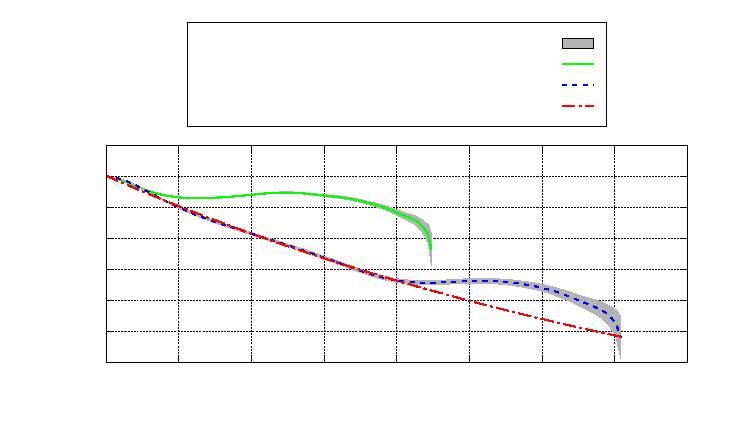
\includegraphics{tangentkorr}}%
    \gplfronttext
  \end{picture}%
\endgroup

    \caption{Tangentkorrelation för en fri sträng (a) och instängd sträng (b) visas. Ett exponentialsamband anpassas med en karakteristisk längd, \emph{persistence length}, som för den fria strängen är $L_\text{p} = \unit[48.63]{\micro m}$.}
    \label{fig:tangentkorr}
\end{figure}

\subsection{Resultat -- (tvåpunktskorrelation)}
\todo[inline]{ev skippa tvåpunktskorrelation?}


Fysikaliska tolkningen av en tvåpunktskorrelationsfunktion är att ge mått på hur snabbt avvikelser från strängens jämviktsläge skingras med tid samt avstånd på strängen. Korrelationen beräknas numeriskt från strängdatan, vilket betraktats i ett godtyckligt antal ekvidistanta diskreta punkter längs strängen, $\Delta s$ är avståndet mellan två efterföljande punkter. Tvåpunktskorrelationen beräknas för data som en normerad kovariansmatris enligt \todo[color=olive]{referera till eq från stoc. kap}. Temporala korrelationen fås genom att studera strängens utveckling i bildspelet, där $\Delta t$ svarar mot tidsintervallet mellan två följande bilder. Kovariansmatrisen härleddes även teoretiskt för strängar begränsade av mikrokanaler \eqref{2korr}. Den teoretiska korrelationen  beräknas för samma temporala samt rumsliga förskjutningar $\Delta s, \Delta t$ som i strängdatan fås den att helt bestämmas av parametrarna $\gamma,\xi,\sigma$. Genom att matcha dessa olika kovariansmatriser erhålls ett mycket överbestämt ekvationssystem ur vilket dessa parametrar kan bestämmas.
\todo{fixa 3D-plots på dessa och förklara deras utseende} \\ \\
Tvåpunktskorrelationen kan även betraktas i två specialfall; då $\Delta t=0$, vilket likt den minimalisktiska WLC modellen svarar mot korrelation längs strängen, samt då $\Delta s=0$, vilket ger temporal korrelation. För båda fallen kan \eqref{2korr} lösas analytiskt, korrelationen längs strängen ges av
\begin{equation}\label{eq:tangentkorr}
\ev{A(s)A(s')}=\exp(-\sqrt{\frac{\gamma}{\xi}}\abs{\Delta s}),
\end{equation}
vilket är samma som tangentkorrelationen \eqref{tangkorr} för minimalistiska WLC-modellen. Motsvarigheten till $L_{\text{p}}$ för en sträng i en mikrokanal som $L_\text{p}=\sqrt{\frac{\xi}{\gamma}}$.
Temporala korrelationen ges av
\begin{equation}
    \ev{A(t)A(t')}=\mathrm{erfc}(\sqrt{\gamma\abs{\Delta t}}),
\end{equation}
där $\mathrm{erfc}(.)$ är \emph{complementary error function} definerad som $\mathrm{erfc}(x)=\frac{2}{\sqrt{\pi}}\int_{x}^{\infty}\ee^{-y^2}\dd y$.

I figur \todo[color=olive]{figur på 2-korr för confined strängar}.. ses ytor svarandes mot tvåpunktskorrelationerna, där den teoretiska modellen anpassats med avseende på parametrarna $\gamma,\xi,\sigma$ för att matcha numeriska korrelationen. 



\section{Egenmoder -- Cosinustransform}
Ett vanligt sätt att studera svängningar är att dela upp dem i egenmoder. Genom en linjärkombination av dessa egenmoder kan en godtycklig svängning representeras. Anledningen till att det är intressant att studera egenmoder är på grund av att de är oberoende av varandra. Precis som svängningen på en gitarrsträng kan strängens svängningar i cellen eventuellt representeras som en linjärkombination av dess egenmoder. 
Återigen betrakta \eqref{mikrokanel}, då denna modell beskriver strängens svängningar kan det tänkas att dess lösningar kan uttryckas i en sådan linjärkombination. Alltså att positionsvektorn kan utvecklas i en bas av egenmoder
\begin{equation}
\label{basutv}
    A(t,s)=\sum_{n=1}^{\infty}a_{n}(t)\psi_{n}(s),
\end{equation}
där $a_{n}(t)$ är egenvärdet till respektive egenmod $\psi_{n}(s)$. Värdet på $a_{n}(t)$ svarar mot egenmodens amplitud vilket ansätts vara tidsberoende. Insättning i \eqref{mikrokanel} ger följande differentialekvation
\begin{equation}\label{egenvard}
    \gamma\sum_{n=1}^{\infty}\partial_{t}a_{n}(t)\psi_{n}(s)=\kbT\sum_{n=1}^{\infty}a_{n}(t)\left[-L_{\text{p}}\partial_{s}^{4}+\frac{2\mu}{L_{\text{p}}}\partial_{s}^{2}-\frac{\nu}{L_{\text{p}}^{3}}\right]\psi_{n}(s)+\sigma\partial_{t}W(t,s).
\end{equation}
Summanden i högerledet svarar mot en operator verkandes på moderna. Ansätt nu $\psi_{n}(s)$ att vara egenvektorer till operatorn, alltså att
\begin{equation}
    \kbT\left[-L_{\text{p}}\partial_{s}^{4}+\frac{2\mu}{L_{\text{p}}}\partial_{s}^{2}-\frac{\nu}{L_{\text{p}}^{3}}\right]\psi_{n}(s)=\lambda_{n}\psi_{n}(s),
\end{equation}
där $\lambda_{n}$ svarar mot egenvektorernas egenvärden till operatorn vilket antas vara tidsoberoende. Lösningar till denna egenvärdesekvation ges av de trigonometriska funktionerna, dock eftersträvas enbart lösningar vilket samtidigt spänner upp en möjlig bas till strängarnas svängningar. Då strängarnas ändar inte är fixa förkastas \emph{sinus}-delen av lösningen \todo[color=olive]{stämmer detta?}och moderna fås som \cite{PhysRevE.60.4671} $\psi_{n}(s)=\cos({\frac{n\pi}{L}s})$. Insättning av denna i \eqref{egenvard} reducerar ekvationen till en ODE enligt
\begin{equation}
    \sum_{n=1}^{\infty}\left[\gamma\partial_{t}a_{n}(t)+\lambda_{n} a_{n}(t)\right]\psi_{n}(s)=\sigma\partial_{t}W(t,s).
\end{equation}
Medelvärdesbildas ekvationen över tid fås högerledet som $\ev{\sigma\partial_{t}W(t,s)}=0$. Alltså fås det att
\begin{equation}
    \sum_{n=1}^{\infty}\ev{\gamma\partial_{t}a_{n}(t)+\lambda_{n}a_{n}(t)}\psi_{n}(s)=0.
\end{equation}
Då $\psi_{n}(s)$ spänner upp en bas för strängarnas avvikelser är denna icke-trivial, lösningarna till ekvationen fås genom att lösa $\ev{\partial_{t}a_{n}(t)+\lambda a_{n}(t)}=0$. Lösningen till denna differentialekvation ger korrelationsfunktionen för modernas amplituder
\begin{equation}
\label{modkorr2}
    \ev{a_{n}(t)a_{n}(0)}=\ee^{-\frac{\lambda_{n}}{\gamma}t}.
\end{equation}
Det fås att korrelationen för svängningsmoderna avtar exponentiellt med en karakterisktisk tid $\frac{\gamma}{\lambda_{n}}$. För att simplifiera denna ekvationen omdefineras egenvärderna som $\lambda=\frac{\tau_{n}}{\gamma}$, där $\tau_{n}$ är modernas \emph{relaxationstid}. \eqref{modkorr2} fås nu som
\begin{equation}\label{modkorr}
\ev{a_{n}(t)a_{n}(0)}=\ee^{-\frac{t}{\tau_{n}}}.
\end{equation}
Genom att lösa ekvation \eqref{egenvard} för egenmoderna erhålls en ekvation ur vilket tiderna $\tau_{n}$ kan beräknas explicit
\begin{equation}\label{relaxconf}
    \frac{\gamma}{\tau_{n}\kbT}=\frac{2\mu}{L_{\text{p}}}\left(\frac{n\pi}{L}\right)^{2}+L_{\text{p}}\left(\frac{n\pi}{L}\right)^{4}+\frac{\nu}{L_{\text{p}}^3}.
\end{equation}
Relaxationstiden avtar proportionellt mot ordningen på moden  $\tau_{n}\propto\frac{1}{n^4}$. Eftersom den harmoniska potentialen med styrka $\nu$ \todo[color=olive]{stämmer detta samt stycket under fortfarande?}modellerar den begränsande kanalen så ses enligt denna modell att relaxationstiden för högre ordningens moder påverkas mindre av kanalen. 

Samma analys kan göras för strängar vars svängningar inte begränsas av mikrokanalen. Då en sådan sträng inte upplever någon harmonisk potential sätts den modellerande konstanten $\nu\equiv0$ i \eqref{mans}. Lösningsmetoden är analogt till fallet då $\gamma\neq0$ och relaxationstiderna fås att enbart bero på ordningen av moden 
\begin{equation}\label{relaxnonconf}
    \frac{\gamma}{\tau_{n}\kbT}=\frac{2\mu}{L_{\text{p}}}\left(\frac{n\pi}{L}\right)^{2}+L_{\text{p}}\left(\frac{n\pi}{L}\right)^{4}.
\end{equation}


\subsection{Resultat -- }
Enligt \eqref{basutv} kan avståndsvektorn $A(t,s)$, innehållandes strängens transversella fluktuationer, uttryckas i en bas av egenmoder. Tidigare erhölls det att en sådan bas spänns upp av egenvektorerna $\psi_{n}(s)=\cos({\frac{n\pi}{L}s})$ vars egenvärden fås genom diskret cosinustransform av $A(t,s)$. De tidsberoende egenvärdena korreleras och enligt \eqref{modkorr} beräknas modernas relaxationstid då denna är definerad som den takt med vilket korrelationen avtar. I figur \ref{fig:cosconf} ses relaxationstider $\tau$ plottade mot modens vågtal $k$ för strängar inneslutna i en mikrokanal. Figur \ref{fig:cosconf} visar motsvarande data fast för fria strängarna. I överensstämmande med \eqref{relaxconf} och \eqref{relaxnonconf} ses ett snabbt avtagande samband för båda typerna av strängar, alltså att moder med låga vågtal förblir representiva för strängens svängningar under längre tidsperioder.

I figur \ref{fig:cosconf} ses bara relaxationstider för de första 6 moderna. Eftersom den tid vilket en mod förblir exiterad avtar snabbt med dess vågtal, resultat det mindre data att medelvärdera och korrelera. Detta samband kan studeras i figurerna då det syns att felmarginalerna för relaxationstiderna ökar kraftigt med vågtal.




\begin{figure}
    \centerline{
    \subfigure[][]{
    \input{bilder/strangar/cosktauconf.tex}\label{fig:cosconf}
    }
    \subfigure[][]{
    \input{bilder/strangar/cosktaunonconf.tex}\label{fig:cosnonconf}
    }}
    \caption{Dispersionrelation för de första cosinus-moderna. Vardera figur innehåller data från 2 strängar för fria samt instängda strängar. För moder med större vågtal erhölls inget användbart samband, därför plottas enbart de signifikanta moderna för vardera sträng. Felmariginalerna för $\tau$ är satta som 95\,\%-iga konfidensintervall.}
\end{figure}


\section{Egenmoder -- Kovariansmatris}


I tidigare avsnitt undersöktes strängens rörelse genom att utveckla denna i en cosinustransform. En annan netod för sönderläggning av strängens rörelse i egenmoder beskrivs i avsnitt \ref{sec:kovmatris} som en diagonalisering av kovariansmatrisen, där kovariansmatrisen $C$ i detta fallet konstrueras av de transversella avstånden $A_s(t)$. Diagonalisering av denna kovariansmatris med hjälp av spektralsatsen leder effektivt till ett basbyte från en bas bestående av det transversella avståndet i varje punkt $s$ längs strängen, till en bas bestående av egenmoderna för strängen. Egenvärdena till kovariansmatrisen ger ett mått på hur mycket av strängens rörelse som byggs upp av motsvarande egenmod, framtida användning av storleken på moden avser storleken på egenvärdet. I avsnitt \ref{sec:kovmatris} påpekas även att den tidsmedelvärdesbildade variansen av varje mod svarar precis mot egenvärdena till kovariansmatrisen. Genom att projicera strängens rörelse på ett fåtal av de egenmoder med störst egenvärde förenklas analysen\cite{Shlens_PCA2014}; karakteristiska egenskaper för varje egenmod kan undersökas separat. Hädanefter betecknas därför det transversella avståndet till strängen relativt sitt jämviktsläge $A_s(t)$ där $s$ är en \emph{diskret} båglängdsparameter längs med strängen.

Kovariansmatrisen bildad av $A_s(t)$ fås enligt \eqref{eq:kovmatris} som 
\begin{equation}
\label{eq:C}
    C_{ij} = \COV{A_s(t)}{A_{s'}(t)}_t.
\end{equation}
Egenvektorerna till $C$, hädanefter egenmoderna, betecknas $\mathbf{B}_i$ och strängrörelsen kan representeras som
\begin{equation}
    A_s(t) = \sum_i^n \alpha_{si}(t)\mathbf{B_i},
\end{equation}
$\hat{\mathbf{A}}_s$ är en enhetsvektor längs komponent $s$ och 
\begin{equation}
    \alpha_{si}(t) = A_s(t)\mathbf{B}_i\cdot\hat{\mathbf{A}}_s.
\end{equation}
Projektionen av strängrörelsen på varje egenmod som funktion av tiden beskrivs av
\begin{equation}
    b_i(t) = \sum_s^n \alpha_{si}(t).
\end{equation}

Autokorrelationsfunktionen för varje komponent $b_i(t)$ innehåller information om strängrörelsens tidsutveckling. Genom att endast betrakta de komponenter med ''tillräckligt'' stora egenvärden förenklas analysen och relaxationstider för de mest dominanta egenmoderna tas fram från 
\begin{equation}
\label{eq:korrmoder}
    \ev{b_i(t)b_i(t+\Delta t)}_t.
\end{equation}
Antalet egenvärden som är tillräckligt att studera beror på hur väl man vill beskriva rörelsen. Det finns flera modeller för att bestämma hur många egenvärden som behövs, men enligt \cite{Cangelosi2007} så förutspår dessa inte alltid entydiga svar. 


\subsection{Resultat -- Signifikanta egenmoder och avtagande dispersionsrelation}

Egenvärdena, som är precis $\VAR{\mathbf{B}_i}$, till kovariansmatrisen bildad från de stokastiska processerna $A_s(t)$ visas i \figref{fig:kovegenvarde} och en tydlig variation i storlek ses. Den stora skillnaden i varians visar att strängrörelsen till en god approximation kan beskrivas i ett fåtal egenmoder snarare än separata avstånd i varje punkt längs strängen. Vidare visas i \figref{fig:egenmoder} tre typiska egenmoder för strängarna; dessa egenmoder hör till en fri sträng men ingen väsentlig skillnad för egenmoder ses mellan fria och instängda strängar. Egenmoder liknar till viss grad harmoniska svängningar \todo{Harmoniska svängningar eller cosinusvågor? Eller något annat} där den största avvikelsen ses vara vid strängens ändar.

%Antalet egenvärde \sim polynomgrad


För att försöka bestämma ett samband mellan vågtalen och relaxationstiderna, en dispersionrelation, anpassas en cosinusvåg till vardera egenmod för att bestämma modens vågtal. Felgränsen på vågtalet tas fram genom att plotta egenmoden mot andraderivatan av den samma i \figref{fig:osak_vagtal}, för en exakt cosinusvåg väntas en rak linje med lutning $-k^2$; ty $\pd_x^2\cos{kx}=-k^2\cos{kx}$. Genom att anpassa en trendlinje i minsta kvadratmening och mäta standardavvikelsen för anpassningen kan en felgräns uppskattas, vilket används för att bestämma ett 95\, \% konfidensintervall.


\subsubsection{Avtagande dispersionsrelation}
Vidare beräknas för varje separat egenmod en relaxationstid genom korrelationen \eqref{eq:korrmoder} vilket visas för en fri sträng i \figref{fig:korrelation}. Korrelationen ses avta exponentiellt i tiden vilket överensstämmer med \eqref{modkorr} och $\nicefrac{-1}{\tau_i}$ ges av lutningen för motsvarande egenmod. Lutningen ses vara störst för den största moden och sedan minska med modens storlek; vilket alltså svarar mot en ökad relaxationstid för stora egenmoder. 

Slutligen plottas dispersionsrelation för de fyra strängarna i \figref{fig:dispersion}. Det tydligaste resultatet är att relaxationstiden minskar med ökat vågtal. Det finns dock en viss avvikelse från detta för moder med små vågtal. De instängda strängarna visas i \figref{fig:ktauconf} och relaxationstiden för deras egenmoder är i intervallet \unit[0.1--2]{s}. Motsvarande har de fria strängarna i \figref{fig:ktaunonconf} relaxationstider i intervallet \unit[0.1--10]{s}. Således spänner relaxationstiden för de fria strängarna över ett större intervall än för de begränsade strängarna. 
\todo{fetstila B i figur}
\begin{figure}
    \centering
    % GNUPLOT: LaTeX picture with Postscript
\begingroup
  \makeatletter
  \providecommand\color[2][]{%
    \GenericError{(gnuplot) \space\space\space\@spaces}{%
      Package color not loaded in conjunction with
      terminal option `colourtext'%
    }{See the gnuplot documentation for explanation.%
    }{Either use 'blacktext' in gnuplot or load the package
      color.sty in LaTeX.}%
    \renewcommand\color[2][]{}%
  }%
  \providecommand\includegraphics[2][]{%
    \GenericError{(gnuplot) \space\space\space\@spaces}{%
      Package graphicx or graphics not loaded%
    }{See the gnuplot documentation for explanation.%
    }{The gnuplot epslatex terminal needs graphicx.sty or graphics.sty.}%
    \renewcommand\includegraphics[2][]{}%
  }%
  \providecommand\rotatebox[2]{#2}%
  \@ifundefined{ifGPcolor}{%
    \newif\ifGPcolor
    \GPcolortrue
  }{}%
  \@ifundefined{ifGPblacktext}{%
    \newif\ifGPblacktext
    \GPblacktexttrue
  }{}%
  % define a \g@addto@macro without @ in the name:
  \let\gplgaddtomacro\g@addto@macro
  % define empty templates for all commands taking text:
  \gdef\gplbacktext{}%
  \gdef\gplfronttext{}%
  \makeatother
  \ifGPblacktext
    % no textcolor at all
    \def\colorrgb#1{}%
    \def\colorgray#1{}%
  \else
    % gray or color?
    \ifGPcolor
      \def\colorrgb#1{\color[rgb]{#1}}%
      \def\colorgray#1{\color[gray]{#1}}%
      \expandafter\def\csname LTw\endcsname{\color{white}}%
      \expandafter\def\csname LTb\endcsname{\color{black}}%
      \expandafter\def\csname LTa\endcsname{\color{black}}%
      \expandafter\def\csname LT0\endcsname{\color[rgb]{1,0,0}}%
      \expandafter\def\csname LT1\endcsname{\color[rgb]{0,1,0}}%
      \expandafter\def\csname LT2\endcsname{\color[rgb]{0,0,1}}%
      \expandafter\def\csname LT3\endcsname{\color[rgb]{1,0,1}}%
      \expandafter\def\csname LT4\endcsname{\color[rgb]{0,1,1}}%
      \expandafter\def\csname LT5\endcsname{\color[rgb]{1,1,0}}%
      \expandafter\def\csname LT6\endcsname{\color[rgb]{0,0,0}}%
      \expandafter\def\csname LT7\endcsname{\color[rgb]{1,0.3,0}}%
      \expandafter\def\csname LT8\endcsname{\color[rgb]{0.5,0.5,0.5}}%
    \else
      % gray
      \def\colorrgb#1{\color{black}}%
      \def\colorgray#1{\color[gray]{#1}}%
      \expandafter\def\csname LTw\endcsname{\color{white}}%
      \expandafter\def\csname LTb\endcsname{\color{black}}%
      \expandafter\def\csname LTa\endcsname{\color{black}}%
      \expandafter\def\csname LT0\endcsname{\color{black}}%
      \expandafter\def\csname LT1\endcsname{\color{black}}%
      \expandafter\def\csname LT2\endcsname{\color{black}}%
      \expandafter\def\csname LT3\endcsname{\color{black}}%
      \expandafter\def\csname LT4\endcsname{\color{black}}%
      \expandafter\def\csname LT5\endcsname{\color{black}}%
      \expandafter\def\csname LT6\endcsname{\color{black}}%
      \expandafter\def\csname LT7\endcsname{\color{black}}%
      \expandafter\def\csname LT8\endcsname{\color{black}}%
    \fi
  \fi
    \setlength{\unitlength}{0.0500bp}%
    \ifx\gptboxheight\undefined%
      \newlength{\gptboxheight}%
      \newlength{\gptboxwidth}%
      \newsavebox{\gptboxtext}%
    \fi%
    \setlength{\fboxrule}{0.5pt}%
    \setlength{\fboxsep}{1pt}%
\begin{picture}(6802.00,4534.00)%
    \gplgaddtomacro\gplbacktext{%
      \csname LTb\endcsname%
      \put(980,640){\makebox(0,0)[r]{\strut{}$10^{-17}$}}%
      \csname LTb\endcsname%
      \put(980,2467){\makebox(0,0)[r]{\strut{}$10^{-13}$}}%
      \csname LTb\endcsname%
      \put(980,4293){\makebox(0,0)[r]{\strut{}$10^{-9}$}}%
      \csname LTb\endcsname%
      \put(1100,440){\makebox(0,0){\strut{}$0$}}%
      \csname LTb\endcsname%
      \put(2089,440){\makebox(0,0){\strut{}$5$}}%
      \csname LTb\endcsname%
      \put(3078,440){\makebox(0,0){\strut{}$10$}}%
      \csname LTb\endcsname%
      \put(4067,440){\makebox(0,0){\strut{}$15$}}%
      \csname LTb\endcsname%
      \put(5056,440){\makebox(0,0){\strut{}$20$}}%
      \csname LTb\endcsname%
      \put(6045,440){\makebox(0,0){\strut{}$25$}}%
    }%
    \gplgaddtomacro\gplfronttext{%
      \csname LTb\endcsname%
      \put(160,2466){\rotatebox{-270}{\makebox(0,0){\strut{}var[$\mathbf{B}_i$] /[m$^2$]}}}%
      \put(3770,140){\makebox(0,0){\strut{}$\lambda_k$}}%
      \csname LTb\endcsname%
      \put(5778,4065){\makebox(0,0)[r]{\strut{}Instängd sträng nr. 1}}%
      \csname LTb\endcsname%
      \put(5778,3845){\makebox(0,0)[r]{\strut{}Instängd sträng nr. 2}}%
      \csname LTb\endcsname%
      \put(5778,3625){\makebox(0,0)[r]{\strut{}Fri sträng nr. 1}}%
      \csname LTb\endcsname%
      \put(5778,3405){\makebox(0,0)[r]{\strut{}Fri sträng nr. 2}}%
    }%
    \gplbacktext
    \put(0,0){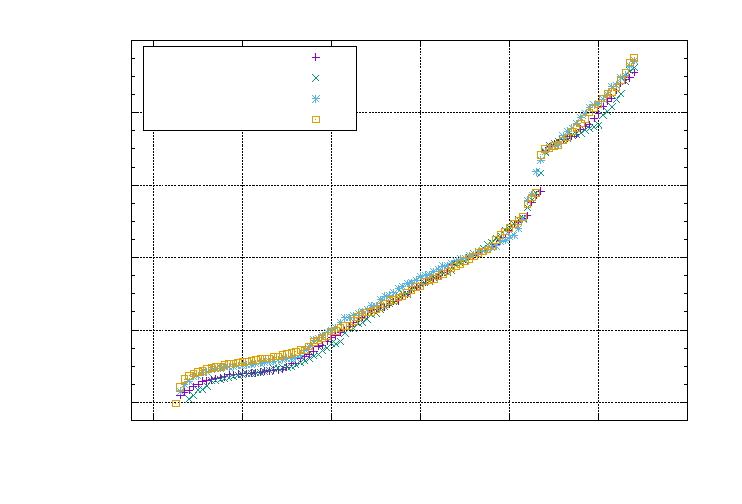
\includegraphics{kovegenv}}%
    \gplfronttext
  \end{picture}%
\endgroup

    \caption{De största egenvärdena till kovariansmatrisen från \eqref{eq:C} för de fyra strängarna som studerats. Det ses att $\VAR{B_i}$ varierar stort då $\VAR{B_1}/\VAR{B_{20}}\approx10^7$. Icke visade egenvärden avtar exponentiellt och dessa moder bidrar inte signifikant till strängens rörelse.}
    \label{fig:kovegenvarde}
\end{figure}
\todo{subplotta moder och dess fel? Åtminstone felen kanske onödigt att det tar upp så stor yta?}
\begin{figure}
    \centering
    \input{bilder/strangar/moder.tex}
    \caption{Typiska egenmoder för en sträng. Dessa egenmoder hör till en fri sträng men inga väsentliga skillnader för egenmodernas utseende fanns mellan fria och instängda strängar. Det ses att delar av egenmoderna liknar harmoniska svängningar; avvikelse från dessa är störst vid ändarna på strängen.}
    \label{fig:egenmoder}
\end{figure}


\begin{figure}
    \centering
    \input{bilder/strangar/osak_vagtal.tex}
    \caption{Samband mellan $v_i(l)$ och $\frac{\pd^2v_i (l)}{\pd l^2}$ för att bestämma osäkerheten i anpassat vågtal. För en egenmod som är en exakt cosinusvåg väntas en rak linje med lutning $-k^2$; avvikelserna från en sådan linje antyder om hur mycket egenmoden avviker från en cosinusvåg.}
    \label{fig:osak_vagtal}
\end{figure}

\begin{figure}
    \centering
    % GNUPLOT: LaTeX picture with Postscript
\begingroup
  \makeatletter
  \providecommand\color[2][]{%
    \GenericError{(gnuplot) \space\space\space\@spaces}{%
      Package color not loaded in conjunction with
      terminal option `colourtext'%
    }{See the gnuplot documentation for explanation.%
    }{Either use 'blacktext' in gnuplot or load the package
      color.sty in LaTeX.}%
    \renewcommand\color[2][]{}%
  }%
  \providecommand\includegraphics[2][]{%
    \GenericError{(gnuplot) \space\space\space\@spaces}{%
      Package graphicx or graphics not loaded%
    }{See the gnuplot documentation for explanation.%
    }{The gnuplot epslatex terminal needs graphicx.sty or graphics.sty.}%
    \renewcommand\includegraphics[2][]{}%
  }%
  \providecommand\rotatebox[2]{#2}%
  \@ifundefined{ifGPcolor}{%
    \newif\ifGPcolor
    \GPcolortrue
  }{}%
  \@ifundefined{ifGPblacktext}{%
    \newif\ifGPblacktext
    \GPblacktexttrue
  }{}%
  % define a \g@addto@macro without @ in the name:
  \let\gplgaddtomacro\g@addto@macro
  % define empty templates for all commands taking text:
  \gdef\gplbacktext{}%
  \gdef\gplfronttext{}%
  \makeatother
  \ifGPblacktext
    % no textcolor at all
    \def\colorrgb#1{}%
    \def\colorgray#1{}%
  \else
    % gray or color?
    \ifGPcolor
      \def\colorrgb#1{\color[rgb]{#1}}%
      \def\colorgray#1{\color[gray]{#1}}%
      \expandafter\def\csname LTw\endcsname{\color{white}}%
      \expandafter\def\csname LTb\endcsname{\color{black}}%
      \expandafter\def\csname LTa\endcsname{\color{black}}%
      \expandafter\def\csname LT0\endcsname{\color[rgb]{1,0,0}}%
      \expandafter\def\csname LT1\endcsname{\color[rgb]{0,1,0}}%
      \expandafter\def\csname LT2\endcsname{\color[rgb]{0,0,1}}%
      \expandafter\def\csname LT3\endcsname{\color[rgb]{1,0,1}}%
      \expandafter\def\csname LT4\endcsname{\color[rgb]{0,1,1}}%
      \expandafter\def\csname LT5\endcsname{\color[rgb]{1,1,0}}%
      \expandafter\def\csname LT6\endcsname{\color[rgb]{0,0,0}}%
      \expandafter\def\csname LT7\endcsname{\color[rgb]{1,0.3,0}}%
      \expandafter\def\csname LT8\endcsname{\color[rgb]{0.5,0.5,0.5}}%
    \else
      % gray
      \def\colorrgb#1{\color{black}}%
      \def\colorgray#1{\color[gray]{#1}}%
      \expandafter\def\csname LTw\endcsname{\color{white}}%
      \expandafter\def\csname LTb\endcsname{\color{black}}%
      \expandafter\def\csname LTa\endcsname{\color{black}}%
      \expandafter\def\csname LT0\endcsname{\color{black}}%
      \expandafter\def\csname LT1\endcsname{\color{black}}%
      \expandafter\def\csname LT2\endcsname{\color{black}}%
      \expandafter\def\csname LT3\endcsname{\color{black}}%
      \expandafter\def\csname LT4\endcsname{\color{black}}%
      \expandafter\def\csname LT5\endcsname{\color{black}}%
      \expandafter\def\csname LT6\endcsname{\color{black}}%
      \expandafter\def\csname LT7\endcsname{\color{black}}%
      \expandafter\def\csname LT8\endcsname{\color{black}}%
    \fi
  \fi
    \setlength{\unitlength}{0.0500bp}%
    \ifx\gptboxheight\undefined%
      \newlength{\gptboxheight}%
      \newlength{\gptboxwidth}%
      \newsavebox{\gptboxtext}%
    \fi%
    \setlength{\fboxrule}{0.5pt}%
    \setlength{\fboxsep}{1pt}%
\begin{picture}(6802.00,3968.00)%
    \gplgaddtomacro\gplbacktext{%
      \csname LTb\endcsname%
      \put(980,640){\makebox(0,0)[r]{\strut{}$10^{-13}$}}%
      \csname LTb\endcsname%
      \put(980,1669){\makebox(0,0)[r]{\strut{}$10^{-12}$}}%
      \csname LTb\endcsname%
      \put(980,2698){\makebox(0,0)[r]{\strut{}$10^{-11}$}}%
      \csname LTb\endcsname%
      \put(980,3727){\makebox(0,0)[r]{\strut{}$10^{-10}$}}%
      \csname LTb\endcsname%
      \put(1100,440){\makebox(0,0){\strut{}$0$}}%
      \csname LTb\endcsname%
      \put(2435,440){\makebox(0,0){\strut{}$0,5$}}%
      \csname LTb\endcsname%
      \put(3771,440){\makebox(0,0){\strut{}$1$}}%
      \csname LTb\endcsname%
      \put(5106,440){\makebox(0,0){\strut{}$1,5$}}%
      \csname LTb\endcsname%
      \put(6441,440){\makebox(0,0){\strut{}$2$}}%
    }%
    \gplgaddtomacro\gplfronttext{%
      \csname LTb\endcsname%
      \put(160,2183){\rotatebox{-270}{\makebox(0,0){\strut{}$\ev{b_{i}(t)b_{i}(t+\Delta t)}$}}}%
      \put(3770,140){\makebox(0,0){\strut{}$\Delta t$ /[s]}}%
      \csname LTb\endcsname%
      \put(2580,1055){\makebox(0,0)[r]{\strut{}$\tau_1=\unit[7,24]{s}$}}%
      \csname LTb\endcsname%
      \put(2580,835){\makebox(0,0)[r]{\strut{}$\tau_2=\unit[2,52]{s}$}}%
      \csname LTb\endcsname%
      \put(4179,1055){\makebox(0,0)[r]{\strut{}$\tau_3=\unit[1,16]{s}$}}%
      \csname LTb\endcsname%
      \put(4179,835){\makebox(0,0)[r]{\strut{}$\tau_4=\unit[0,61]{s}$}}%
      \csname LTb\endcsname%
      \put(5778,1055){\makebox(0,0)[r]{\strut{}$\tau_5=\unit[0,31]{s}$}}%
      \csname LTb\endcsname%
      \put(5778,835){\makebox(0,0)[r]{\strut{}$\tau_6=\unit[0,32]{s}$}}%
    }%
    \gplbacktext
    \put(0,0){\includegraphics{korrfil3}}%
    \gplfronttext
  \end{picture}%
\endgroup

    \caption{Korrelationen \eqref{fig:korrmoder} för de sex största egenmoderna, där egenmodernas storlek avtar med $i$. Ett exponentiellt samband ses mellan korrelationen och tiden. En linje anpassas i minsta-kvadrat mening och lutningen $a_i$ ger relaxationstiden enligt $\tau_i=\nicefrac{1}{\abs{a_i}}$. Relaxationstiderna för moderna ges i figuren.}
    \label{fig:korrelation}
\end{figure}





\begin{figure}\centerline{
\subfigure[][]{
\input{bilder/strangar/ktauconf.tex}\label{fig:ktauconf}
}
\subfigure[][]{
\input{bilder/strangar/ktaunonconf.tex}\label{fig:ktaunonconf}
}}
\caption{Dispersionsrelation för strängarnas olika egenmoder. Bortsett från vissa moder med lågt $k$ så minskar relaxationstiden med ökande vågtal. Felmariginalerna för $\tau$ är satta som 95\,\%-iga konfidensintervall; för $k$ är de bara uppskattade genom att undersöka hur anpassningen försämras om man ändrar $k$.}
\label{fig:dispersion}
\end{figure}


%Resultat som kan tas med

%Motivera att jämviktsläge fanns
%Uppdelningen i egenmoder, olika relaxationstid
%Dispersionsrelation?
%Skillnad mellan confined och unconfined



\section{Diskussion}

Nedan finns förslag på rubriker, ändra gärna och lägg till

\subsection{Polynomanpassningens påverkan på resultatet}

\subsection{Strängen verkar vibrera kring ett jämviktläge}

\subsection{Skillnad mellan fria och instängda strängar}
Den tydligaste skillnaden mellan fria och instängda strängar är skillnaden i relaxationstiden för de olika egenmoderna vilket visades i \figref{fig:dispersion}. Att relaxationstiden för de fria strängarna spänner över ett större intervall anses rimligt, detta eftersom de är just fria; de begränsas inte av en kanal vilket torde göra att dess form är mer beständig i tiden.  



\subsection{hur $L_\text{p}>>L_\text{sträng}$ påverkar resultaten}

\subsection{Egenmoder från kovariansmatrisen}
Att variansen för egenmoderna framtagna från kovariansmatrisen sprider sig över ett extremt stort intervall ($\sim 10^7$ för de $20$ största av totalt $128$) är en tydlig indikation på att strängens rörelse till en god grad kan representeras av okorrelerade egenmoder, snarare än representeras av korrelerande avståndskomponenter. Däremot är antalet egenmoder med signifikant varians korrelerad med gradantalet på de till strängarna anpassade polynomen. Så en för stor vikt ska inte läggas på det specifika antalet. Även inom dessa $20$ största egenmoder så ska det noteras att huvudsakligen analyseras bara ett fåtal av dessa, exempelvis maximalt $7$\,st för beräkning av vågtal samt relaxationstid. Såldes anses inte valet av polynomgraden ha någon inverkan på de presenterade resultaten. 

Att egenvektorerna från kovariansmatrisen uppvisar ett beteende likt vad som förväntas för harmonisk rörelse är fascinerande\todo{Är fascinerande. Är det för ''personligt''? Är noterbart kanske?}.  

\subsection{Avtagande dispersionsrelation}
Relaxationstiden för egenmoderna visades avta med ökat vågtal, mer specifikt skulle man kunna tänkas anpassa en trendlinje i logplottarna från \figref{fig:dispersion}. Dock ses en avvikelse från detta för vissa låga vågtal vilket gör det svårt att motivera en sådan anpassningen. Vidare hade mätdatan för fler egenmoder behövts för att motivera en anpassning. Problematiken med att undersöka fler moder är att framtagen korrelation \eqref{modkorr} för egenmoder i \figref{fig:korrelation} endast har få mätpunkter i det exponentiella området; relaxationstiden för egenmoder med högre vågtal är för liten. Detta eftersom upplösningen på kameran som filmat strängarna var 10 bilder per sekund, samtidigt ses relaxationstiden för egenmoderna med stort vågtal vara i storleksordningen \unit[0.1]{s}. För att undersöka egenmoder med högre vågtal behövs alltså strängarna studeras med en högre tidsupplösning vilket skulle möjliggöra fler mätpunkter i det exponentiella området.

\subsection{Cosinustransform eller utveckling i egenmoder från kovmatris}
%Varför avviker egenmoder från kovmatris från cosvågor. Kan tänkas bero på att strängarnas fluktationer inte är homogen, mer svängning vid de lösa ändarna. 
Anledningen till att studera strängens rörelse både genom cosinustranform samt egenmoder framtagna från kovariansmatrisen var huvudsakligen av två skäl. Cosinustransformens fördel är att vågtalen för cosinusvågorna är exakt bestämda, till skillnad mot egenmoderna från kovariansmatrisen vars form ej nödvändigtvis behöver likna cosinusvågor vilket gör beräkning av vågtalet icke-trivialt. %skriva mer här

Fördelen med att använda egenmoderna framtagna från kovariansmatrisen är att variansen av egenmoderna ger ett mått på hur mycket av rörelsen som representeras av just den egenmoden. Därför kan 




%Bara en liten kodsnutt som behövs när man kompilerar lokalt
%%% Local Variables: 
%%% mode: latex
%%% TeX-master: "00main.tex"
%%% End: 